La verifica dei contratti software non esaurisce la valutazione di un agente.
Un workflow può rispettare gli schemi e produrre una risposta scorrevole usando
un luogo o un periodo sbagliato. Il progetto adotta quindi un benchmark
ancorato a evidenze, controlli deterministici e un LLM-as-a-Judge. Questo
capitolo descrive il \textbf{protocollo~6.0} implementato in
\path{backend/app/evals/} (versione dichiarata in
\path{dataset/schema.py}) e distingue i conteggi riportati per il dataset corrente dai risultati
storici riscontrabili nella guida allegata. Gli artefatti originali delle run
correnti non sono inclusi nei materiali di questa stesura: i conteggi possono
essere controllati aritmeticamente, ma non ricostruiti caso per caso. Per confronto storico, in chiusura si richiamano anche
le run parziali con protocollo~4.0 documentate nella guida del 15 ottobre 2026
\cite{guidaProgetto2026}; i due insiemi non sono direttamente sommabili perché
differiscono per protocollo, hash del dataset e regole di esito.

\begin{figure}[htbp]
\centering
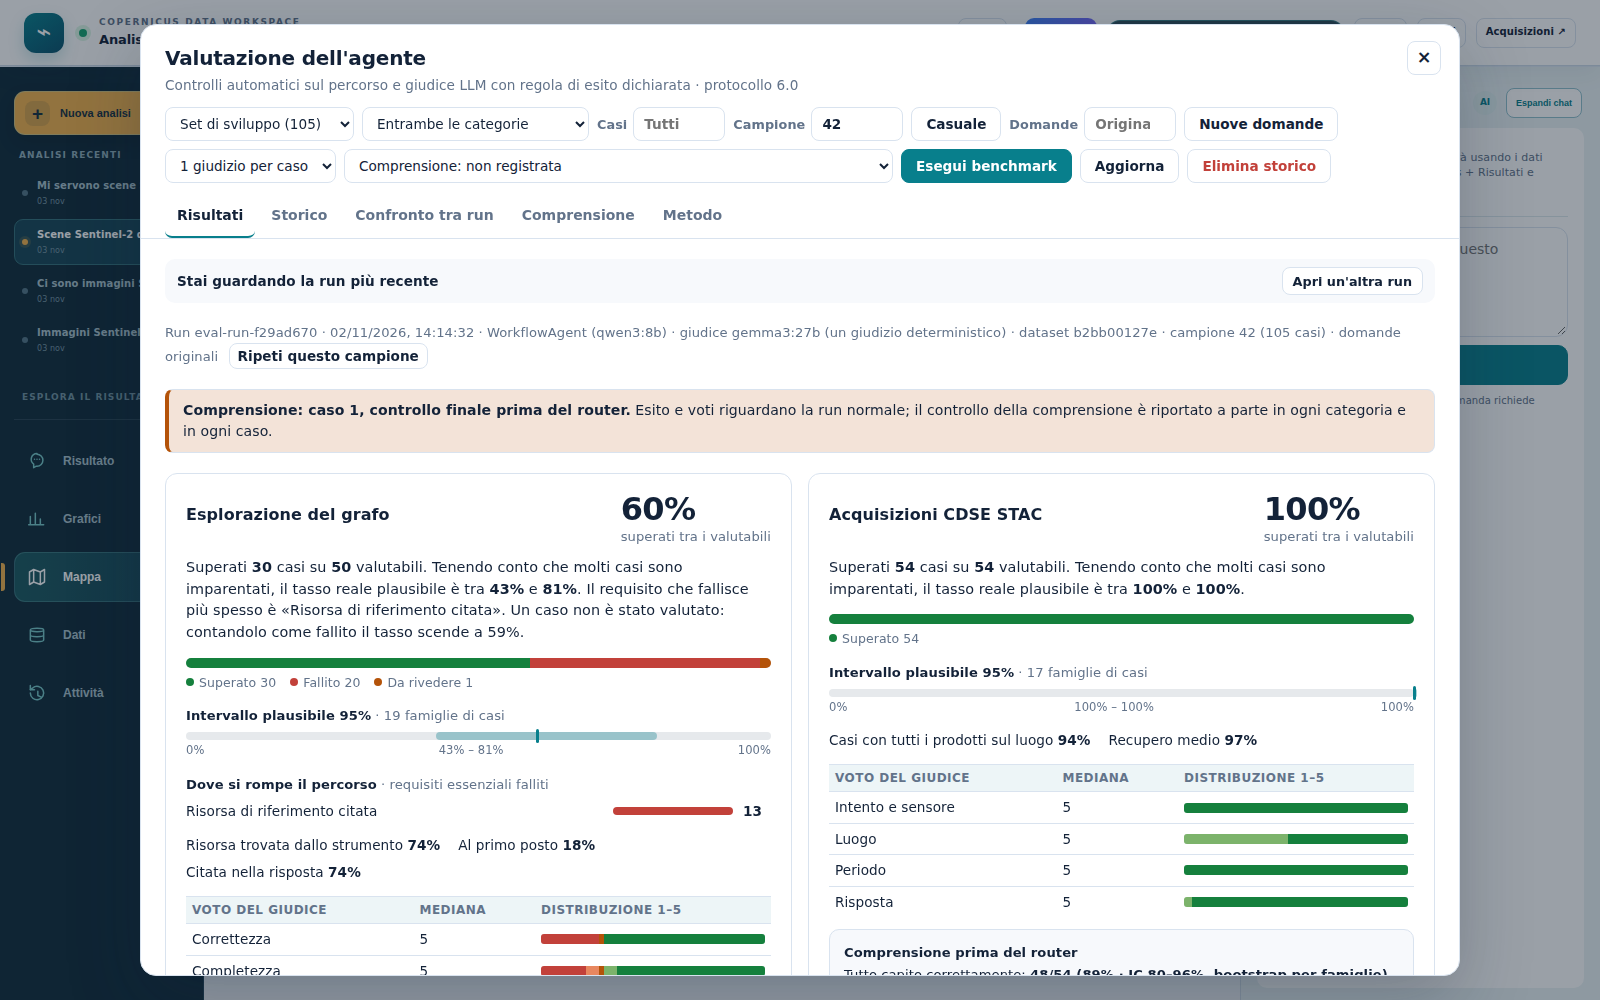
\includegraphics[width=0.88\textwidth]{Images/screenshots/ui-evals-panel.png}
\caption{Schermata illustrativa del pannello di valutazione: dataset, Judge,
controlli e sintesi per categoria. La run mostrata nell'interfaccia non è una
prova dei conteggi della Tabella~\ref{tab:risultati-6}.}
\label{fig:ui-evals-panel}
\end{figure}

\section{Oggetto e perimetro della valutazione}

Il sistema sotto esame è il \texttt{WorkflowAgent}, comprendente instradamento,
interpretazione, recupero e sintesi. Il runner gli sottopone la domanda
originale; il Judge valuta risposta ed evidenze osservate. Nella configurazione
documentata, il modello dell'agente è \texttt{qwen3:8b} e il Judge predefinito è
\texttt{gemma3:27b}. La famiglia diversa riduce una possibile fonte di
preferenza per le proprie risposte, senza garantire imparzialità.

Il Judge non è un modello addestrato nel repository per assegnare voti: viene
interrogato con rubriche e output JSON vincolato. È distinto dal nodo
Verification dell'agente, che appartiene al percorso di esecuzione. La
valutazione a posteriori su casi noti non va confusa con un controllo interno
al singolo turno.

Opzionalmente, il protocollo~6.0 può registrare una validazione della
\emph{comprensione} prima del router, tramite il campo
\texttt{validation\_mode}
con le modalità \texttt{none}, \texttt{self\_report},
\texttt{verifier} o \texttt{stage\_checks}.
L'esito pass/fail del caso resta quello della run ordinaria; le modalità di
comprensione sono uno strato aggiuntivo e non sostituiscono i voti del Judge.

La letteratura evidenzia che i giudizi LLM possono risentire di posizione,
verbosità e preferenza per le proprie famiglie di modelli
\cite{zhengJudge2023}: i voti del Judge vanno quindi letti insieme ai controlli
deterministici e alle misure di incertezza del protocollo. Inoltre il Judge
riceve già l'esito di quei controlli: il voto è \emph{informato} dai fatti
verificati e non costituisce una conferma indipendente degli stessi. Non è
disponibile, in questa tesi, una validazione umana stratificata dei voti sul
compito geospaziale; eventuali falsi pass/fail del Judge restano quindi una
minaccia aperta alla validità.

\section{Dataset ed evidenze di riferimento}

\subsection{Composizione dei casi}

Il dataset corrente \path{backend/app/evals/dataset/benchmark_questions.json}
contiene \textbf{105 casi}: 51 di categoria \texttt{graph} e 54 di categoria
\texttt{acquisitions}, organizzati rispettivamente in 19 e 17 famiglie
(\texttt{cluster}). Ogni caso conserva domanda, risposta attesa, strumenti
attesi, evidenze, tag e famiglia di scenari.

I casi del grafo coprono Marine, Drought e CDSE/STAC catalogati in NebulaGraph.
Le acquisizioni usano collezioni Sentinel-2 L1C/L2A e Sentinel-1 GRD/SLC; alcuni
casi prevedono un risultato vuoto: cercare correttamente e dichiarare l'assenza
di prodotti può costituire un successo. Esiste inoltre un set perturbato
\path{benchmark_perturbed.json}, riservato a prove di generalizzazione e non
usato per tarare le regole.

Questa stratificazione amplia la varietà linguistica ma non rende indipendenti
le parafrasi. Domande sullo stesso luogo possono condividere il medesimo errore
di geocodifica. La numerosità dei casi deve quindi essere accompagnata da
quella delle famiglie effettivamente osservate.

\subsection{Costruzione della ground truth}

Per il grafo, il generatore verifica che titolo, tipo, area, risoluzione e
variabili dichiarati nella domanda siano sostenuti dai metadati della risorsa.
I riscontri sono conservati in \texttt{evidence.grounding}. Un vincolo non
supportato impedisce di trattare il caso come riferimento valido.

Per STAC, il riferimento comprende query con bbox, periodo e collection,
item osservati e identificativi. I \texttt{core\_ids} individuano i prodotti
che coprono il centro del luogo secondo il criterio del benchmark. La loro
copertura misura il recupero di questo insieme di riferimento, senza provare
che sia stato recuperato ogni prodotto esistente nel catalogo.

I riferimenti sono snapshot di metadati. Non includono download di raster o
misure scientifiche sulle variabili. Il catalogo remoto può cambiare: una
differenza di ID rispetto allo snapshot non equivale da sola a un errore
dell'agente e va interpretata insieme alla query e ai prodotti osservati.

\section{Esecuzione del vero workflow}

Il runner invoca \texttt{WorkflowAgent.run\_detailed()} con la domanda originale
e un thread nuovo per ogni caso. Per le acquisizioni richiede
\texttt{include\_eval\_trace=True}, ottenendo interpretazione, query effettiva
e prodotti. L'agente non riceve bbox, sensore o intervallo già risolti dal
riferimento: sostituire il workflow con una chiamata diretta STAC misurerebbe
soltanto il client, lasciando fuori comprensione e routing.

La sequenza comprende esecuzione dell'agente, controlli deterministici,
giudizio, verifica della coerenza dei voti, decisione e salvataggio del JSON
della run. \texttt{used\_tools} deriva dalle sorgenti osservate nel risultato;
\texttt{expected\_tools} resta un requisito del caso. Confondere i due campi
renderebbe invisibile un errore di instradamento.

Il timeout dell'agente è configurabile, con default di 600 secondi. Il campo
\path{execution_time_ms} comprende anche i passaggi valutativi successivi,
incluso il Judge: non rappresenta la sola latenza del workflow in Grafana.
La prova non apre il browser; non certifica quindi la corrispondenza fra
artefatto e tabella o mappa effettivamente visualizzate.

I moduli principali sono \path{runner/engine.py}, \path{runner/checks.py},
\path{judge/prompts.py}, \path{judge/evaluator.py} e \path{stats/metrics.py},
relativi a \path{backend/app/evals/}. Run di protocolli precedenti (4.0/5.0)
non vanno mescolate con le sintesi 6.0 senza dichiarare la versione.

\section{Controlli deterministici e rubriche ordinali}

\subsection{Controlli sui fatti osservati}

I controlli producono esiti vero, falso o non applicabile e una gravità
\texttt{critical}, \texttt{major}, \texttt{minor} o \texttt{info}. Un
fallimento critico impone l'esito negativo. Gli altri sono mostrati al Judge e
riportati nel risultato, ma non sono tutti automaticamente bloccanti.

Per il grafo si verifica che il percorso sia Discovery, senza sostituzione con
web, GDACS, MCP o STAC operativo. Vengono misurati recupero, posizione e
citazione della risorsa di riferimento, oltre ai campi richiesti. La mancata
citazione di un target univoco è critica.

Per le acquisizioni, nel protocollo~6.0 sono critici, fra gli altri: percorso
STAC corretto; luogo, periodo e sensore della query; filtri richiesti sulla
selezione della dashboard; selezione coerente (senza filtri non richiesti
aggiunti dall'agente); risposta live da CDSE (un artefatto in cache dopo una
risposta vuota è errore); assenza di identificativi inventati. Controlli
maggiori riguardano, per esempio, la quota di prodotti sul luogo e la coerenza
della sintesi con i prodotti selezionati.

Se una query corretta incontra un guasto della sorgente, il caso può essere non
valutabile. Un luogo o periodo già errati non vengono invece giustificati dal
guasto successivo.

\subsection{Dimensioni e soglie}

I voti sono interi da 1 a 5 con ancore esplicite per ogni livello. Le rubriche
del protocollo~6.0 differiscono per categoria, come mostra la
Tabella~\ref{tab:rubriche-judge}.

\begin{table}[htbp]
\centering
\small
\begin{tabularx}{\textwidth}{>{\raggedright\arraybackslash}p{0.17\textwidth}
    >{\raggedright\arraybackslash}p{0.24\textwidth}
    >{\raggedright\arraybackslash}X
    >{\centering\arraybackslash}p{0.09\textwidth}}
\toprule
Categoria & Dimensione & Oggetto del giudizio & Soglia \\
\midrule
Grafo & correctness & Correttezza della risorsa e dei vincoli. & 4 \\
 & completeness & Presenza degli elementi richiesti. & 4 \\
 & relevance & Focalizzazione e pertinenza. & 3 \\
 & faithfulness & Assenza di affermazioni false rispetto allo strumento. & 4 \\
\midrule
Acquisizioni & intent & Sensore/prodotto e filtri richiesti. & 4 \\
 & place & Luogo effettivamente interrogato. & 4 \\
 & period & Intervallo effettivamente interrogato. & 4 \\
 & response & Coerenza della sintesi con i prodotti selezionati. & 4 \\
\bottomrule
\end{tabularx}
\caption{Dimensioni ordinali e soglie minime del protocollo~6.0. I controlli
critici si applicano indipendentemente dai voti.}
\label{tab:rubriche-judge}
\end{table}

Per le acquisizioni, ogni errore sostanziale è attribuito a una sola dimensione
(per esempio area troppo ampia $\rightarrow$ \texttt{place}; filtri sbagliati
$\rightarrow$ \texttt{intent}). \texttt{faithfulness} sul grafo misura solo
l'assenza di affermazioni false rispetto all'output dello strumento: una
risposta ``non ho trovato nulla'', quando lo strumento non ha restituito nulla,
può essere fedele anche se scorretta rispetto al riferimento.

La media dei quattro voti è un descrittore e non decide l'esito. Una sequenza
5, 5, 5, 1 ha media 4 ma non supera le soglie.

\subsection{Prompt, parsing e coerenza}

Il Judge riceve domanda, riferimento, risposta, traccia e controlli. Nella
configurazione ordinaria usa temperatura zero, seed fisso, contesto 16.384 token
e output JSON vincolato. Se parsing o voti risultano incoerenti con i fatti
verificati, è previsto un ulteriore tentativo; una contraddizione persistente
viene marcata per revisione (\texttt{review}).

\section{Stati finali e denominatori}

Il protocollo distingue cinque stati:
\begin{description}
    \item[\texttt{pass}] controlli critici rispettati e soglie superate;
    \item[\texttt{fail}] fallimento critico o almeno un voto insufficiente;
    \item[\texttt{review}] incoerenza residua dei voti che richiede esame;
    \item[\texttt{not\_evaluable}] evidenza non utilizzabile, guasto esterno su
    richiesta corretta o valutatore inutilizzabile;
    \item[\texttt{error}] errore, timeout o assenza di risposta dell'agente.
\end{description}

Indicando con $P,F,R,U,E$ i conteggi dei cinque stati, i due tassi sono:
\begin{equation}
 p_{\mathrm{primario}}=\frac{P}{P+F}, \qquad
 p_{\mathrm{rigoroso}}=\frac{P}{P+F+R+U+E}.
\label{eq:tassi-judge}
\end{equation}
Il primo riguarda i casi con esito pass/fail; il secondo include tutti i casi
completati in modo conservativo. Se non esistono casi valutabili, il tasso
primario è assente. In caso di interruzione vengono salvati i casi completati
con \texttt{partial=true}. Le sintesi di grafo e acquisizioni restano separate.

\section{Incertezza e misure di recupero}

\subsection{Intervallo di Wilson}

Per $n=P+F>0$ casi valutabili e proporzione osservata $\hat p=P/n$,
l'intervallo di Wilson al 95\% usa $z\simeq1{,}96$:
\begin{equation}
 \frac{\hat p+z^2/(2n)\ \pm\
 z\sqrt{\hat p(1-\hat p)/n+z^2/(4n^2)}}{1+z^2/n}.
\label{eq:wilson}
\end{equation}
La procedura è disponibile anche nelle librerie statistiche di riferimento
\cite{statsmodelsWilson}. Wilson tratta i casi come osservazioni indipendenti
Bernoulli: non incorpora la dipendenza fra parafrasi della stessa famiglia.
Affiancarlo al bootstrap non ``risolve'' quella dipendenza; i due intervalli
rispondono a ipotesi diverse. Un campione piccolo non sostiene una stima
precisa; l'intervallo non è la probabilità che la prossima risposta sia
corretta.

\subsection{Bootstrap per famiglie e voti ordinali}

Il bootstrap per cluster ricampiona famiglie intere con reinserimento. Si
conserva così la dipendenza interna alle famiglie. Con 17 famiglie di
acquisizioni e 19 di grafo, la varietà effettiva degli scenari conta quanto il
numero di domande. Se tutti i casi passano, il bootstrap può collassare in
$[100\%,100\%]$: è una degenerazione del campione empirico, non una prova di
certezza, e va dichiarata affiancando Wilson e numerosità.

I voti 1--5 sono ordinali. Per ogni dimensione il sistema riporta distribuzione,
mediana e quartili; l'\texttt{overall\_score} medio non sostituisce i singoli
voti né le regole di esito.

\subsection{Indicatori indipendenti dai voti}

Per il grafo si misurano hit, hit@1, citazione e MRR rispetto alla risorsa di
riferimento. Per le acquisizioni si misurano copertura dei \texttt{core\_ids} e
indicatori di recupero sul luogo. Questi indicatori dipendono dalla scelta del
riferimento e non misurano tutta la disponibilità globale del catalogo.

Per interpretare gli indicatori del grafo, si considerino $N>0$ casi e la
posizione $r_i$ del primo risultato pertinente nel caso $i$. Se il riferimento
non è recuperato, si pone $r_i=\infty$ e si assume $1/r_i=0$. Con
$\mathbf{1}[\cdot]$ funzione indicatrice, le definizioni usuali sono:
\[
 \mathrm{hit}=\frac{1}{N}\sum_i\mathbf{1}[r_i<\infty],\qquad
 \mathrm{hit@1}=\frac{1}{N}\sum_i\mathbf{1}[r_i=1],\qquad
 \mathrm{MRR}=\frac{1}{N}\sum_i\frac{1}{r_i}.
\]
La citazione misura separatamente se il riferimento compare nella risposta
finale: presenza nella lista recuperata e menzione nella sintesi non sono
la stessa proprietà. Per le acquisizioni, il richiamo sul riferimento è
il rapporto tra \texttt{core\_ids} recuperati e \texttt{core\_ids} attesi,
quando l'insieme atteso non è vuoto. La quota sul luogo usa invece al
denominatore i prodotti recuperati. Con insiemi vuoti la convenzione deve
essere dichiarata; una media dei rapporti per caso e un rapporto dei totali
non sono intercambiabili. I denominatori effettivi e la gestione delle
esclusioni restano da riscontrare negli artefatti del benchmark.

\section{Confronti e ripetizioni}

\subsection{Riproducibilità e stabilità}

Il campionamento è mescolato con seed. Con una sola ripetizione del Judge la
temperatura è 0; con più ripetizioni (studio di stabilità) è 0,3 e si aggrega
con la mediana per dimensione. Le run registrano protocollo, hash del dataset,
modello Judge, temperatura, seed e numero di ripetizioni, ma non da sole
commit, digest immutabile del modello e stato completo delle sorgenti.

\subsection{Confronti appaiati fra run}

Il confronto ammette run dello \emph{stesso} protocollo, stesso Judge e almeno
20 coppie valutabili per categoria, verificando domanda, evidenza e risposta
attesa dei casi comuni. Wilcoxon signed-rank e McNemar (con correzione di Holm
sulle dimensioni) sono gli strumenti previsti
\cite{scipyWilcoxon,mcnemar1947,statsmodelsHolm}. La soglia delle 20 coppie non
elimina la dipendenza fra famiglie di scenari. Wilcoxon richiede inoltre
ipotesi sulla distribuzione delle differenze, inclusa la simmetria sotto
l'ipotesi nulla, e attenzione a pareggi e zeri, frequenti nei voti 1--5.
Il suo uso sui voti presuppone che le differenze numeriche siano
interpretabili: la sola natura ordinale non garantisce questa proprietà.
Per McNemar vanno considerate le coppie discordanti dell'esito binario.
La famiglia di ipotesi alla quale applicare Holm deve essere dichiarata e
non coincide con le famiglie di parafrasi del dataset. Prima di attribuire
un cambiamento a una modifica è utile un confronto A/A della stessa versione.

\section{Risultati riportati e provenienza}
\label{sec:risultati-judge}

\subsection{Riepilogo riportato per il protocollo~6.0}

Per il dataset descritto da 105 casi, il riepilogo utilizzato nella stesura
attribuisce alla run \texttt{eval-run-ca004ba5} i conteggi della
Tabella~\ref{tab:risultati-6}, con protocollo~6.0, Judge \texttt{gemma3:27b},
temperatura zero e seed 40. Sono risultati riportati, non una nuova esecuzione.
Il file JSON della run, il dataset con il relativo hash e la revisione del
codice non sono allegati; la guida del 15 ottobre documenta invece run del
protocollo~4.0. Non è quindi possibile usare quella guida come prova dei
conteggi correnti o della selezione di questa run rispetto ad altre.
La tabella conserva il riepilogo distinguendo il controllo dei calcoli dalla
verifica sperimentale, che richiede gli artefatti originali.

\begin{table}[htbp]
\centering
\small
\begin{tabularx}{\textwidth}{>{\raggedright\arraybackslash}p{0.22\textwidth}
    >{\centering\arraybackslash}X
    >{\centering\arraybackslash}X
    >{\centering\arraybackslash}X
    >{\centering\arraybackslash}p{0.16\textwidth}}
\toprule
Categoria & Pass (primario) & Pass (rigoroso) & Wilson 95\% & Bootstrap 95\% \\
\midrule
Grafo & 31/49 (63,3\%) & 31/51 (60,8\%) & 49,3--75,3\% & 43,8--81,8\% \\
\addlinespace
Acquisizioni & 54/54 (100\%) & 54/54 (100\%) & 93,4--100\% & 100--100\% \\
\bottomrule
\end{tabularx}
\caption{Conteggi riportati per la run \texttt{eval-run-ca004ba5}, da
riscontrare sugli artefatti originali. Il tasso primario esclude i due
\texttt{review} del grafo; il rigoroso li include nel denominatore. Wilson sui
casi valutabili non incorpora la dipendenza fra famiglie; il bootstrap al
100\% sulle acquisizioni è degenerato (nessun fallimento da ricampionare).}
\label{tab:risultati-6}
\end{table}

La differenza tra i due tassi del grafo dipende dai due casi indicati come
\texttt{review}: il primario esclude questi casi, il rigoroso li include.
L'intervallo Wilson è ricalcolabile dai conteggi; il bootstrap riportato non
è ricostruibile senza famiglie, esiti individuali e configurazione.

Per analizzare i fallimenti è necessario distinguere almeno quattro cause:
instradamento errato, mancato recupero del riferimento, esclusione nel ranking
e risposta finale incompleta o non fedele. Una risorsa alternativa corretta
richiede inoltre una valutazione distinta dall'assenza del target previsto.
La distribuzione di queste cause non viene quantificata in assenza della
traccia originale: la sola presenza di 18 fail non ne identifica l'origine.

Hit, hit@1, MRR, citazione e recupero dei \texttt{core\_ids} devono essere
ricostruiti sulla stessa popolazione di casi, dichiarando esclusioni e
riferimenti. La precisione geografica e il richiamo hanno significati diversi:
se tre prodotti recuperati sono tutti pertinenti e il riferimento ne contiene
sei, la quota pertinente può essere 1 mentre il richiamo è 0,5. Questo è un
esempio illustrativo, non l'esito verificato di un caso del benchmark.
Un pass del protocollo non dimostra quindi esaustività, e l'assenza di
fallimenti bloccanti non elimina eventuali avvisi di qualità.

\subsection{Confronto storico con protocollo~4.0}

La guida del 15 ottobre 2026 documenta run con protocollo~4.0 su un dataset da
115 casi (hash diverso). La più ampia, \texttt{7dc4eda3}, è parziale
(102/115) e riporta 49/51 sul grafo e 32/51 sulle acquisizioni
\cite{guidaProgetto2026}. Il contrasto con la Tabella~\ref{tab:risultati-6}
non dimostra da solo un ``peggioramento'' o un ``miglioramento'' del sistema:
cambiano protocollo, regole critiche, composizione del dataset e completezza
della run. Serve soltanto a collocare storicamente quelle cifre e a evitare di
presentarle come risultato del protocollo corrente.

\section{Interpretazione e minacce alla validità}

Il contributo valutativo consiste nel rendere ispezionabili domanda, evidenze,
percorso, controlli e voti, distinguendo fallimenti dell'agente, problemi
esterni e giudizi inutilizzabili. Wilson e bootstrap descrivono incertezza sotto
ipotesi dichiarate; non correggono un Judge sistematicamente errato.

La validità interna risente di euristiche dei controlli, riduzione delle
evidenze e dipendenze fra casi. La validità esterna rimane limitata da domande
curate, numerosità delle famiglie e snapshot. Per rafforzare le conclusioni
servono confronti A/A, più scenari indipendenti e verifica dell'interfaccia
del workspace, che il benchmark a thread nuovo non osserva.
